
\section{Algorithmic Performance on All Datasets}\label{sec:algorithm_performance}
    For more details on each sample, please see Table \ref{tab:sample_overview}.

\subsection{Results for AGP}
    
    We analyzed three different sample workups of \nglycans released from Alpha 1 Acid
    Glycoprotein. See Table~\ref{tab:agp_parameter_estimates} for a comparison of estimated $\tau$
    values for each sample. For \dpagp and \rpagp, we used an $MS^n$ Signature Ion Criterion
    threshold of 0.17 to filter out large contaminants that may be introduced by permethylation
    reagents.

    The estimate of $\gamma$ for \agp was larger than the score for the larger penta-antennary 

    \begin{table}[h]
        \centering
        \small
        \begin{tabular}{l SSS}
            \toprule
            $\tau_i$ & {\agp} & {\dpagp} & {\rpagp}\\
            \midrule
            high-mannose & 0.000 & 0.000 & 0.000\\
            hybrid & 11.520 & 7.240 & 21.092\\
            bi-antennary & 15.691 & 12.859 & 20.627\\
            asialo-bi-antennary & 0.000 & 0.000 & 13.253\\
            tri-antennary & 21.752 & 21.693 & 21.550\\
            asialo-tri-antennary & 0.000 & 0.000 & 6.792\\
            tetra-antennary & 15.993 & 15.276 & 17.452\\
            asialo-tetra-antennary & 0.000 & 0.000 & 0.000\\
            penta-antennary & 11.446 & 10.127 & 7.282\\
            asialo-penta-antennary & 0.000 & 0.000 & 0.000\\
            hexa-antennary & 2.211 & 0.000 & 0.000\\
            asialo-hexa-antennary & 0.000 & 0.000 & 0.000\\
            hepta-antennary & 0.000 & 0.000 & 0.000\\
            asialo-hepta-antennary & 0.000 & 0.000 & 0.000\\
            \midrule
            ${\hat \lambda}$ & 0.99 & 0.99 & 0.99\\
            ${\hat \gamma}$ & 15.74 & 16.22 & 17.64\\
            \bottomrule
        \end{tabular}
        \caption{Estimated values of smoothing parameters $\tau$, $\lambda$, and $\gamma$ for each
                 AGP-based dataset and using a combinatorial database \label{tab:agp_parameter_estimates}}
    \end{table}

    \begin{figure}[htb]
        \centering
        \begin{minipage}{1\linewidth}
            \centering
            \begin{subfigure}[b]{0.49\linewidth}
                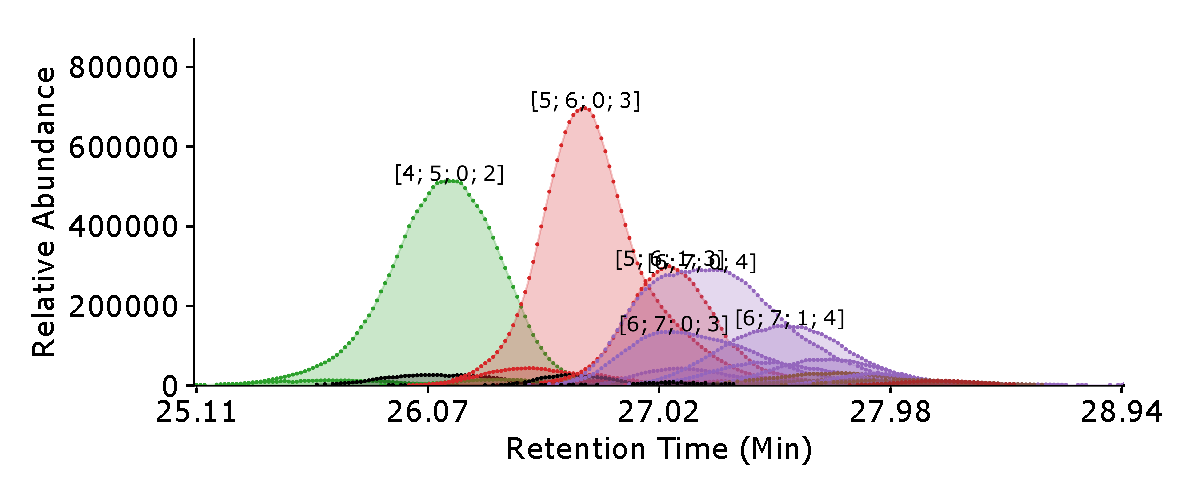
\includegraphics[width=1\linewidth, valign=t]{figure/native_agp_chromatograms.eps}
                \subcaption{
                    \label{fig:agp_assignment:a}
                }
            \end{subfigure}
            \vspace{0pt}
            \begin{subfigure}[b]{0.49\linewidth}
                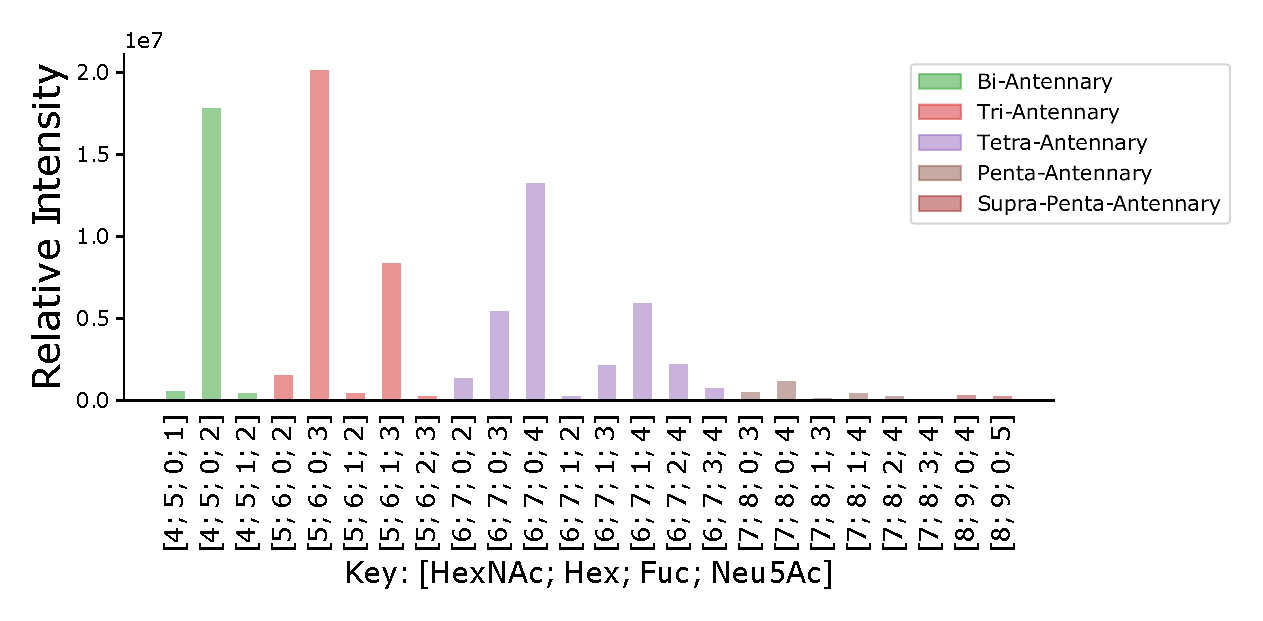
\includegraphics[width=1\linewidth, valign=b]{figure/native_agp_abundances.eps}
                \subcaption{
                    \label{fig:agp_assignment:b}
                }
            \end{subfigure}
        \end{minipage}
        \begin{minipage}{1\linewidth}
            \centering
            \begin{subfigure}[b]{0.49\linewidth}
                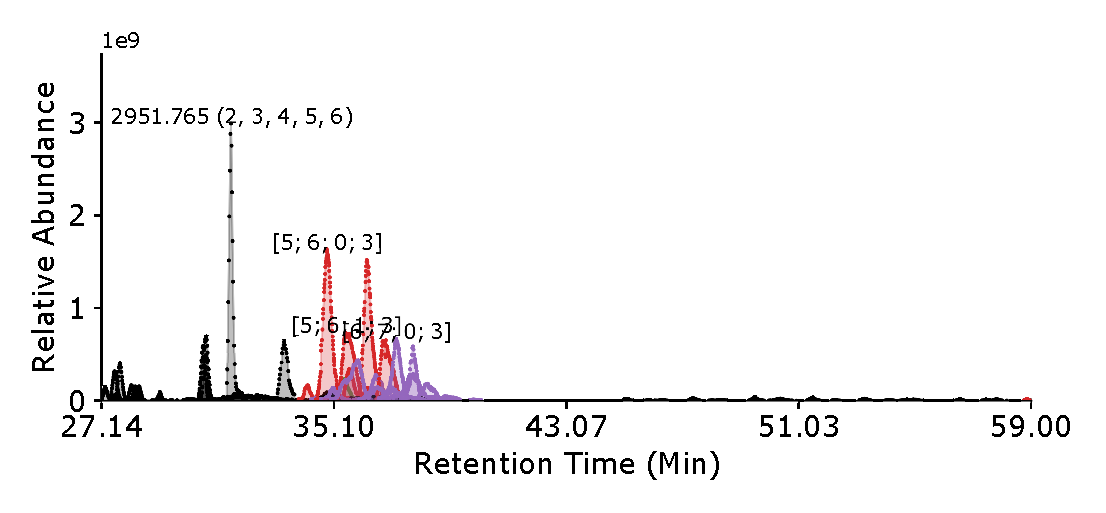
\includegraphics[width=1\linewidth, valign=t]{figure/dp_agp_chromatograms.eps}
                \subcaption{
                    \label{fig:agp_assignment:c}
                }
            \end{subfigure}
            \vspace{0pt}
            \begin{subfigure}[b]{0.49\linewidth}
                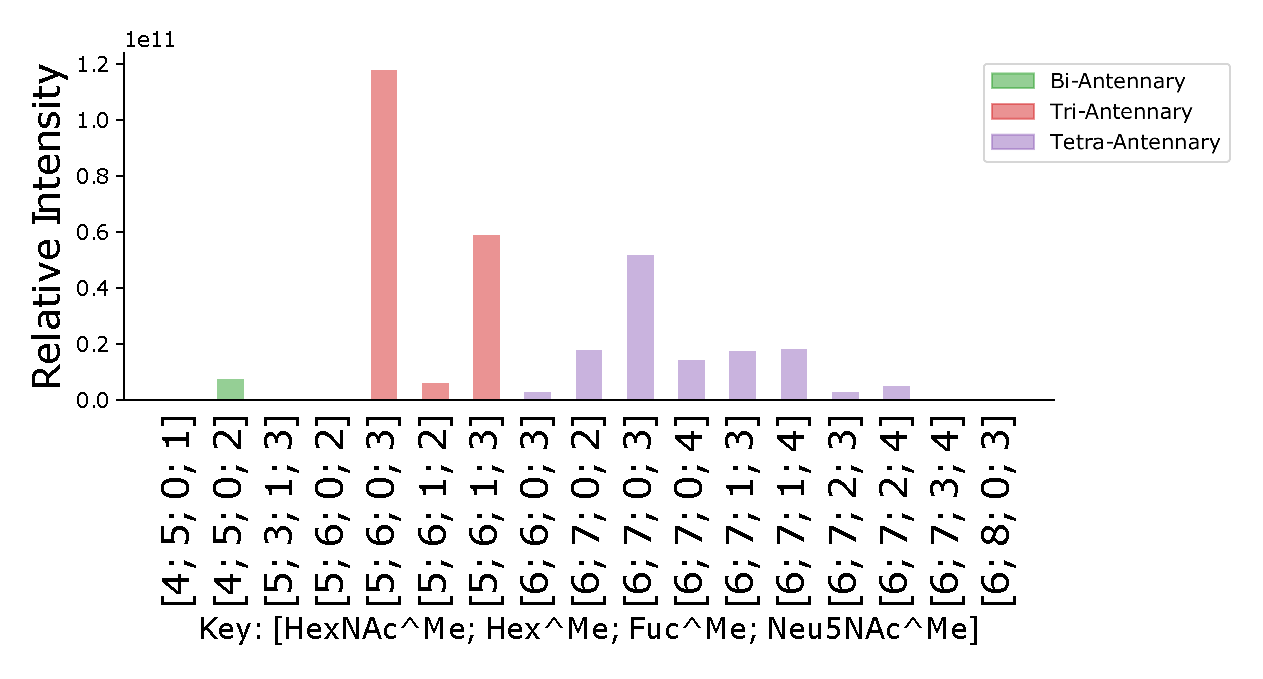
\includegraphics[width=1\linewidth, valign=b]{figure/dp_agp_abundances.eps}
                \subcaption{
                    \label{fig:agp_assignment:d}
                }
            \end{subfigure}
        \end{minipage}
        \begin{minipage}{1\linewidth}
            \centering
            \begin{subfigure}[b]{0.49\linewidth}
                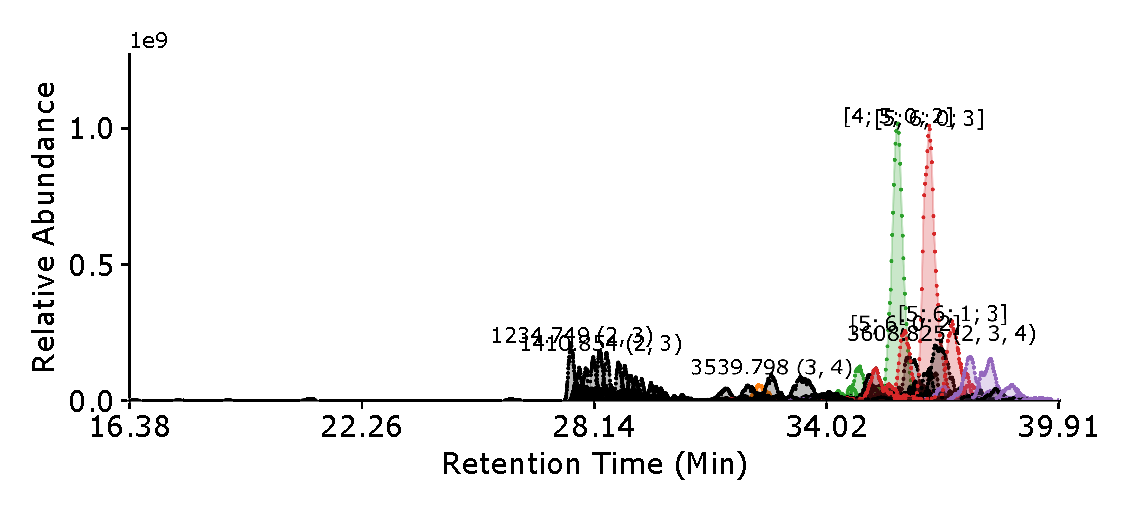
\includegraphics[width=1\linewidth, valign=t]{figure/rp_agp_chromatograms.eps}
                \subcaption{
                    \label{fig:agp_assignment:e}
                }
            \end{subfigure}
            \vspace{0pt}
            \begin{subfigure}[b]{0.49\linewidth}
                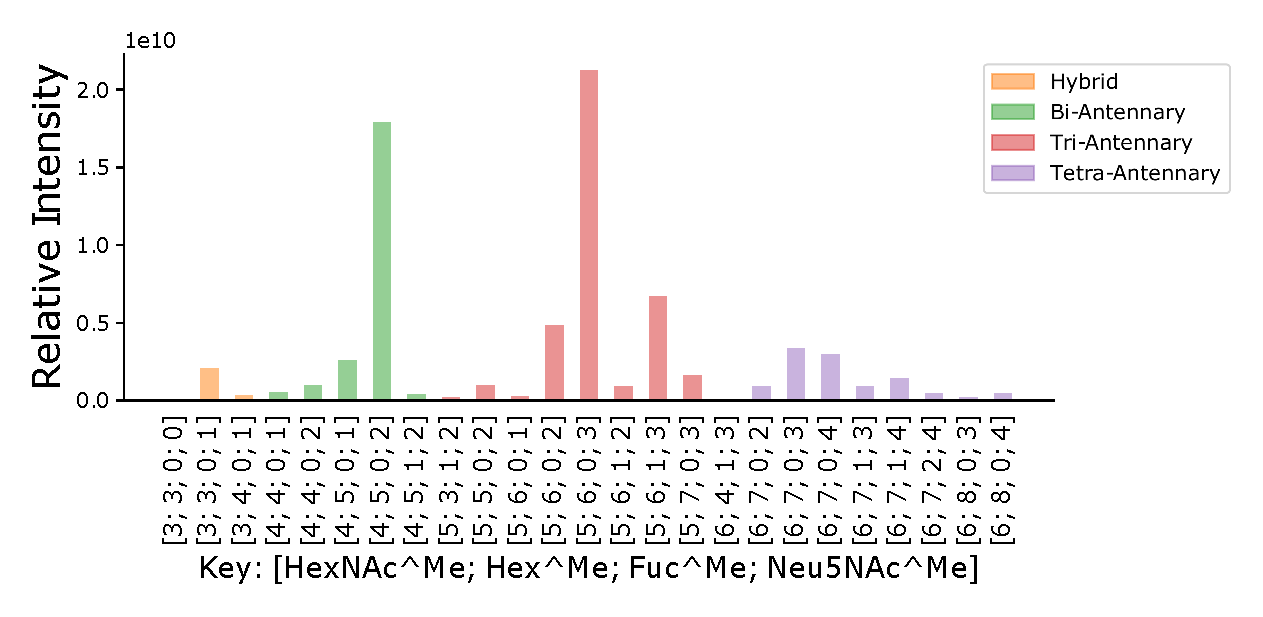
\includegraphics[width=1\linewidth, valign=b]{figure/rp_agp_abundances.eps}
                \subcaption{
                    \label{fig:agp_assignment:f}
                }
            \end{subfigure}
        \end{minipage}
        \caption{Chromatogram Assignments for \agp (a, b), \dpagp (c, d) and \rpagp (e, f)
            \label{fig:agp_assignments}
        }
    \end{figure}
    \FloatBarrier

\subsection{Results for Phil-82}

    We analyzed native and deutero-reduced and permethylated \nglycans released from
    virions of Influenza-A Virus strain Phillipines 1982, both samples acquired on a QTOF
    mass spectrometer. See Table~\ref{tab:phil82_parameter_estimates}
    for a comparison of estimated $\tau$ values for each sample. In the case of \dpphil,
    \msn scans were acquired, resulting in lower resolution chromatographic peaks. We observed
    little ammonium adduction in \dpphil. As expected, we observed abundant formate adduction in
    \phil, particularly on the high mannose glycans. \dpphil also displays considerable in-source
    fragmentation of the high mannose series, defined by the multimodal chromatographic peaks of
    smaller high mannose glycans appearing in lower abundance directly under larger peaks for
    high mannose glycans. This fragmentation, combined with permethylation altering the ionization
    efficiency of these analytes, makes a direct comparison of glycan composition abundance between
    \phil and \dpphil inadvisable. We observe markedly different peak shapes between \phil and \dpphil
    but the relative order of elution is preserved, with the largest high mannose glycans eluting
    later than the largest observed complex type.

    \begin{table}[h]
        \centering
        \small
        \begin{tabular}{l SS}
            \toprule
            $\tau_i$ & {\phil} & {\dpphil}\\
            \midrule
            high-mannose & 17.070 & 19.395\\
            hybrid & 14.039 & 17.147\\
            bi-antennary & 0.000 & 0.000\\
            asialo-bi-antennary & 16.287 & 17.689\\
            tri-antennary & 0.000 & 0.000\\
            asialo-tri-antennary & 15.220 & 18.865\\
            tetra-antennary & 0.000 & 0.000\\
            asialo-tetra-antennary & 7.103 & 7.660\\
            penta-antennary & 0.000 & 0.000\\
            

            asialo-penta-antennary & 0.000 & 3.365\\
            hexa-antennary & 0.000 & 0.000\\
            asialo-hexa-antennary & 0.000 & 0.000\\
            hepta-antennary & 0.000 & 0.000\\
            asialo-hepta-antennary & 0.000 & 0.000\\
            \midrule
            ${\hat \lambda}$ & 0.99 & 0.99\\
            ${\hat \gamma}$ & 16.51 & 15.50\\
            \bottomrule
        \end{tabular}
        \caption{Estimated values of smoothing parameters $\tau$, $\lambda$, and $\gamma$ for each
                 Phil-82-based dataset and using a combinatorial database \label{tab:phil82_parameter_estimates}}
    \end{table}

    \begin{figure}[tb]
        \centering
        \begin{minipage}{1\linewidth}
            \centering
            \begin{subfigure}[b]{0.49\linewidth}
                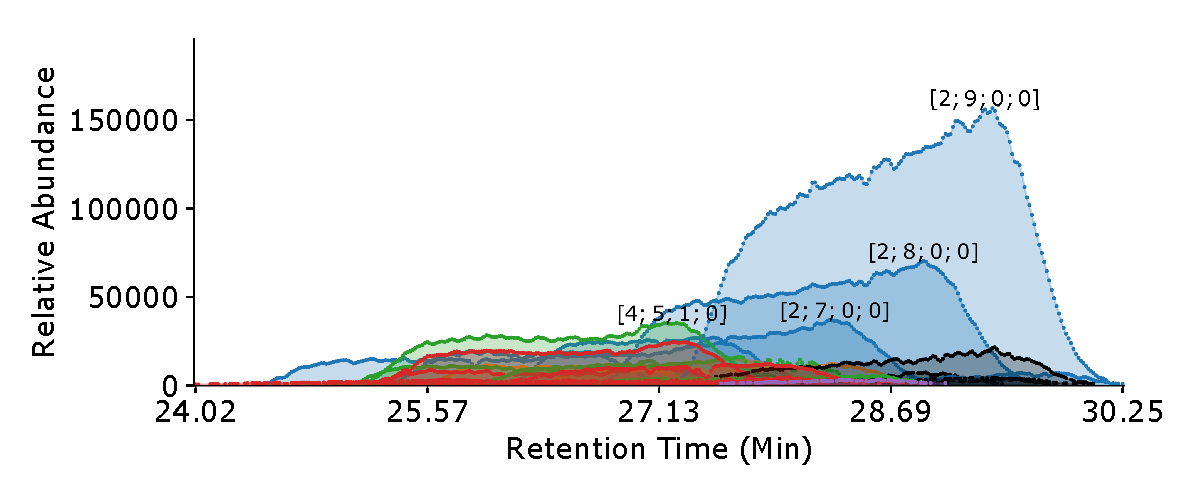
\includegraphics[width=1\linewidth, valign=t]{figure/native_phil82_chromatograms.eps}
                \subcaption{
                    \label{fig:phil82_assignment:a}
                }
            \end{subfigure}
            \vspace{0pt}
            \begin{subfigure}[b]{0.49\linewidth}
                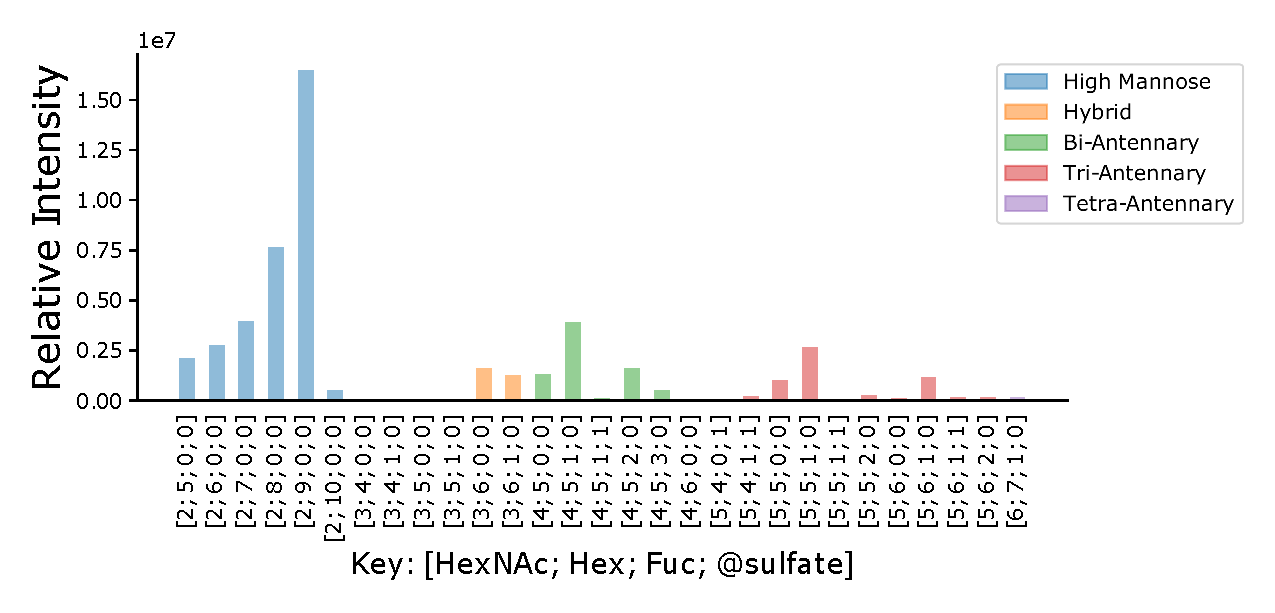
\includegraphics[width=1\linewidth, valign=b]{figure/native_phil82_abundances.eps}
                \subcaption{
                    \label{fig:phil82_assignment:b}
                }
            \end{subfigure}
        \end{minipage}
        \begin{minipage}{1\linewidth}
            \centering
            \begin{subfigure}[b]{0.49\linewidth}
                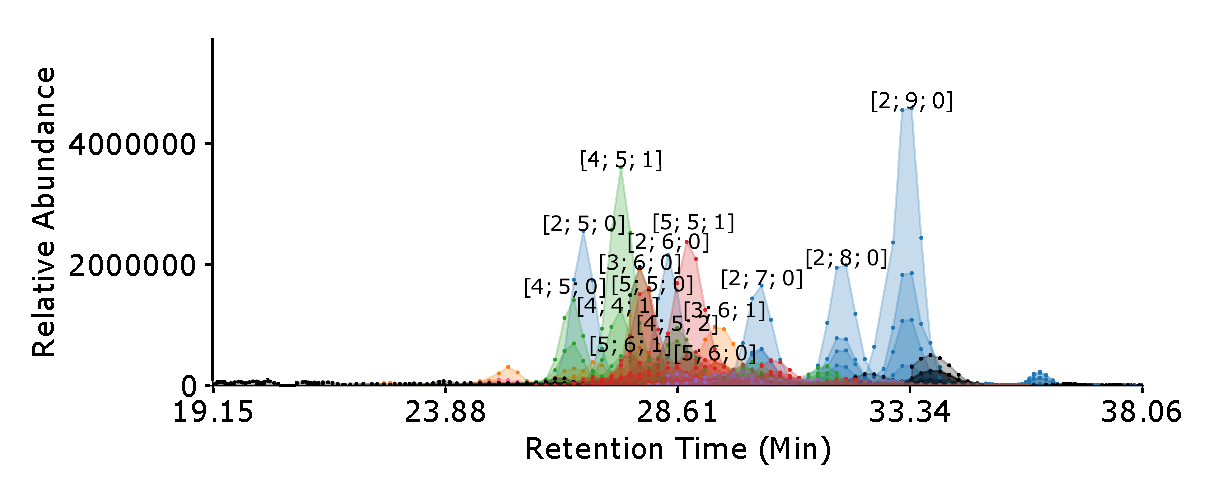
\includegraphics[width=1\linewidth, valign=t]{figure/dp_phil82_chromatograms.eps}
                \subcaption{
                    \label{fig:phil82_assignment:c}
                }
            \end{subfigure}
            \vspace{0pt}
            \begin{subfigure}[b]{0.49\linewidth}
                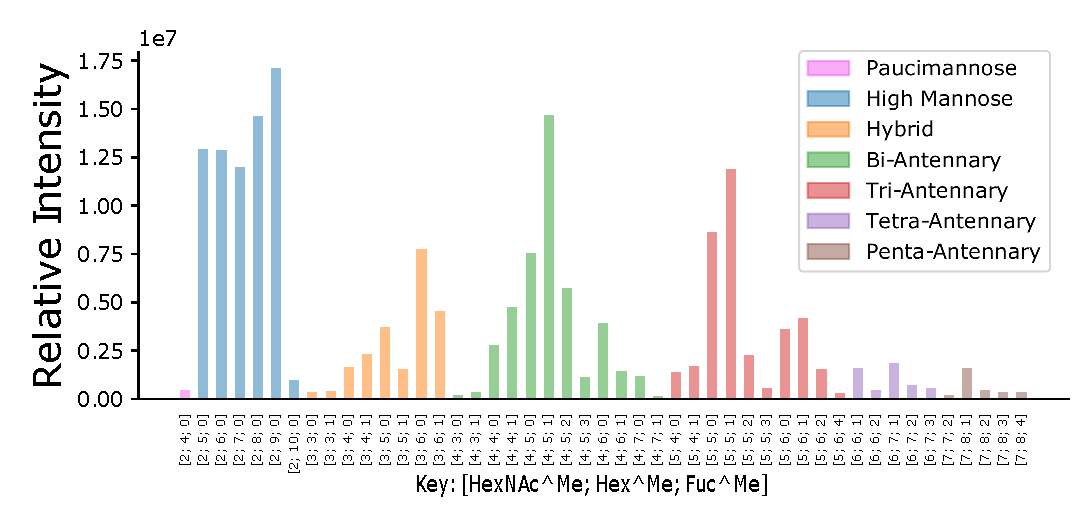
\includegraphics[width=1\linewidth, valign=b]{figure/dp_phil82_abundances.eps}
                \subcaption{
                    \label{fig:phil82_assignment:d}
                }
            \end{subfigure}
        \end{minipage}
        \caption{Chromatogram Assignments for \phil (a, b) and \dpphil (c, d)
            \label{fig:phil82_assignments}
        }
    \end{figure}

\FloatBarrier
\subsection{Results for IGG}
    We analyzed native \nglycans released from IgG. The estimated $\tau$ values shown in
    Table~\ref{tab:igg_parameter_estimates}are consistent with the expectation that IgG
    glycans will be either hybrid or small complex-type structures. These findings are
    consistent with the results from \citealp{Peltoniemi2013}, though their study used
    different sample preparation and instrumentation, and their data were not available
    for side-by-side comparison. The EICs and integrated abundances for this sample are
    shown in Figure~\ref{fig:igg_assignments}.
    
    \begin{table}[h]
        \centering
        \small
        \begin{tabular}{l S}
            \toprule
            $\tau_i$ & {\igg}\\
            \midrule
            high-mannose & 0.000\\
            hybrid & 15.737\\
            bi-antennary & 12.594\\
            asialo-bi-antennary & 13.614\\
            tri-antennary & 7.657\\
            asialo-tri-antennary & 15.724\\
            tetra-antennary & 4.252\\
            asialo-tetra-antennary & 0.000\\
            penta-antennary & 0.000\\
            asialo-penta-antennary & 0.000\\
            hexa-antennary & 0.000\\
            asialo-hexa-antennary & 0.000\\
            hepta-antennary & 0.000\\
            asialo-hepta-antennary & 0.000\\
            \midrule
            ${\hat \lambda}$ & 0.99\\
            ${\hat \gamma}$ & 14.12\\
            \bottomrule
        \end{tabular}
        \caption{Estimated values of smoothing parameters $\tau$, $\lambda$, and $\gamma$ for
                 IGG using a combinatorial database \label{tab:igg_parameter_estimates}}
    \end{table}

    \begin{figure}[htb]
        \centering
        \begin{minipage}{1\linewidth}
            \centering
            \begin{subfigure}[b]{0.49\linewidth}
                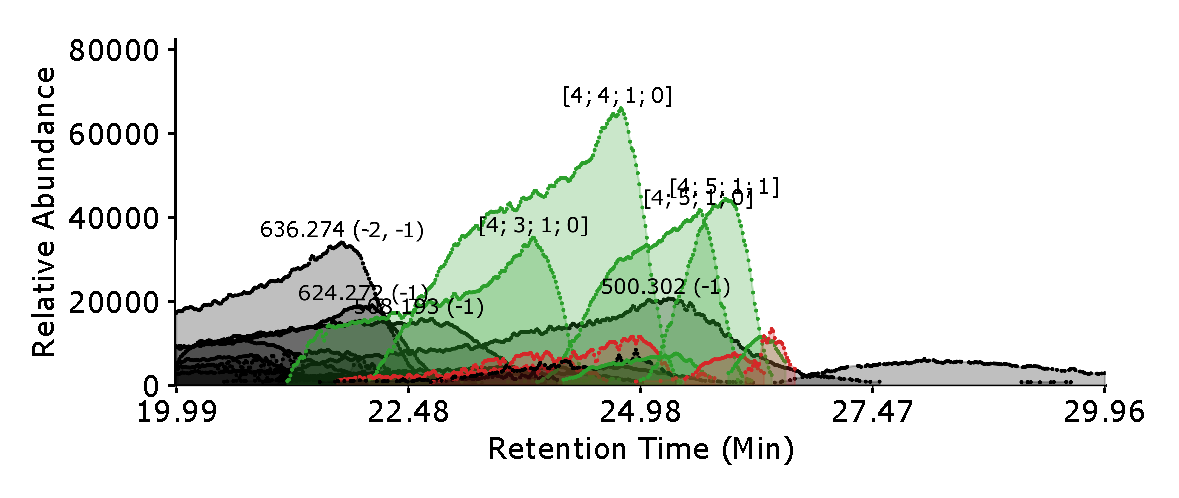
\includegraphics[width=1\linewidth, valign=t]{figure/native_igg_chromatograms.eps}
                \subcaption{
                    \label{fig:igg_assignment:a}
                }
            \end{subfigure}
            \vspace{0pt}
            \begin{subfigure}[b]{0.49\linewidth}
                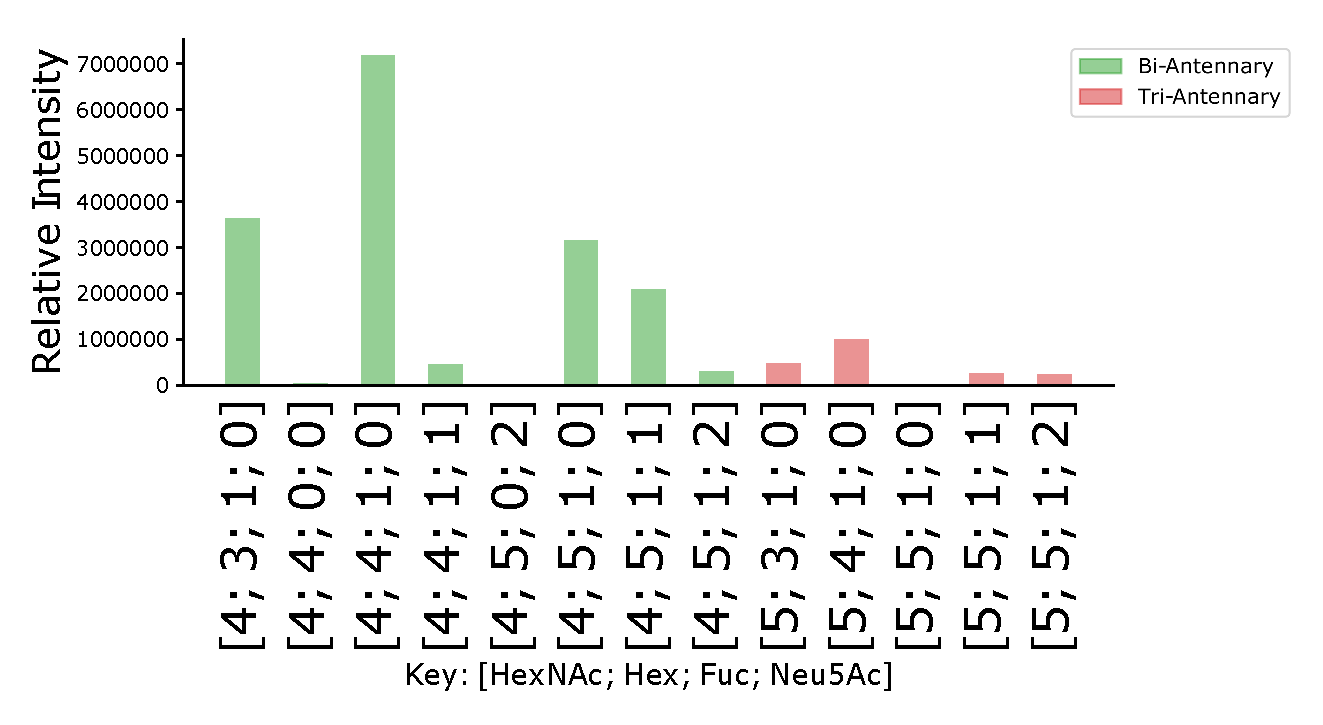
\includegraphics[width=1\linewidth, valign=b]{figure/native_igg_abundances.eps}
                \subcaption{
                    \label{fig:igg_assignment:b}
                }
            \end{subfigure}
        \end{minipage}
        \caption{Chromatogram Assignments for \igg
            \label{fig:igg_assignments}
        }
    \end{figure}
